\section{Introduction}
\label{sec:intro}

因線上外送平台如 Foodpanda 和 UberEat 的迅速發展,餐飲產業的數位化轉型日益顯著。這些平台不僅簡化了顧客與餐廳之間的聯繫,還透過大規模數據分析來改進用戶體驗及提高平台的經濟效益。餐廳推薦系統在這一過程中扮演了至關重要的角色,能夠根據使用者的歷史消費行為、偏好和時下趨勢,及時推薦合適的餐廳,從而提升平台服務的精確性和客戶滿意度。

傳統的推薦系統方法,如基於內容的過濾~(content-based filtering)~和協同過濾~(collaborative filtering)~,雖然在一定程度上能夠提供有效的推薦,但往往忽視了用戶與餐廳之間更深層次的聯繫結構。隨著圖神經網路~(Graph Neural Networks; GNN)~的發展,發現可以將平台上用戶與餐廳之間的關聯性表示為圖結構,從而在更高層次上捕捉到它們之間的複雜互動,其中這個圖結構能以二分圖~(bipartite graph)~表示。
\begin{figure}[tbh]
    \centering
    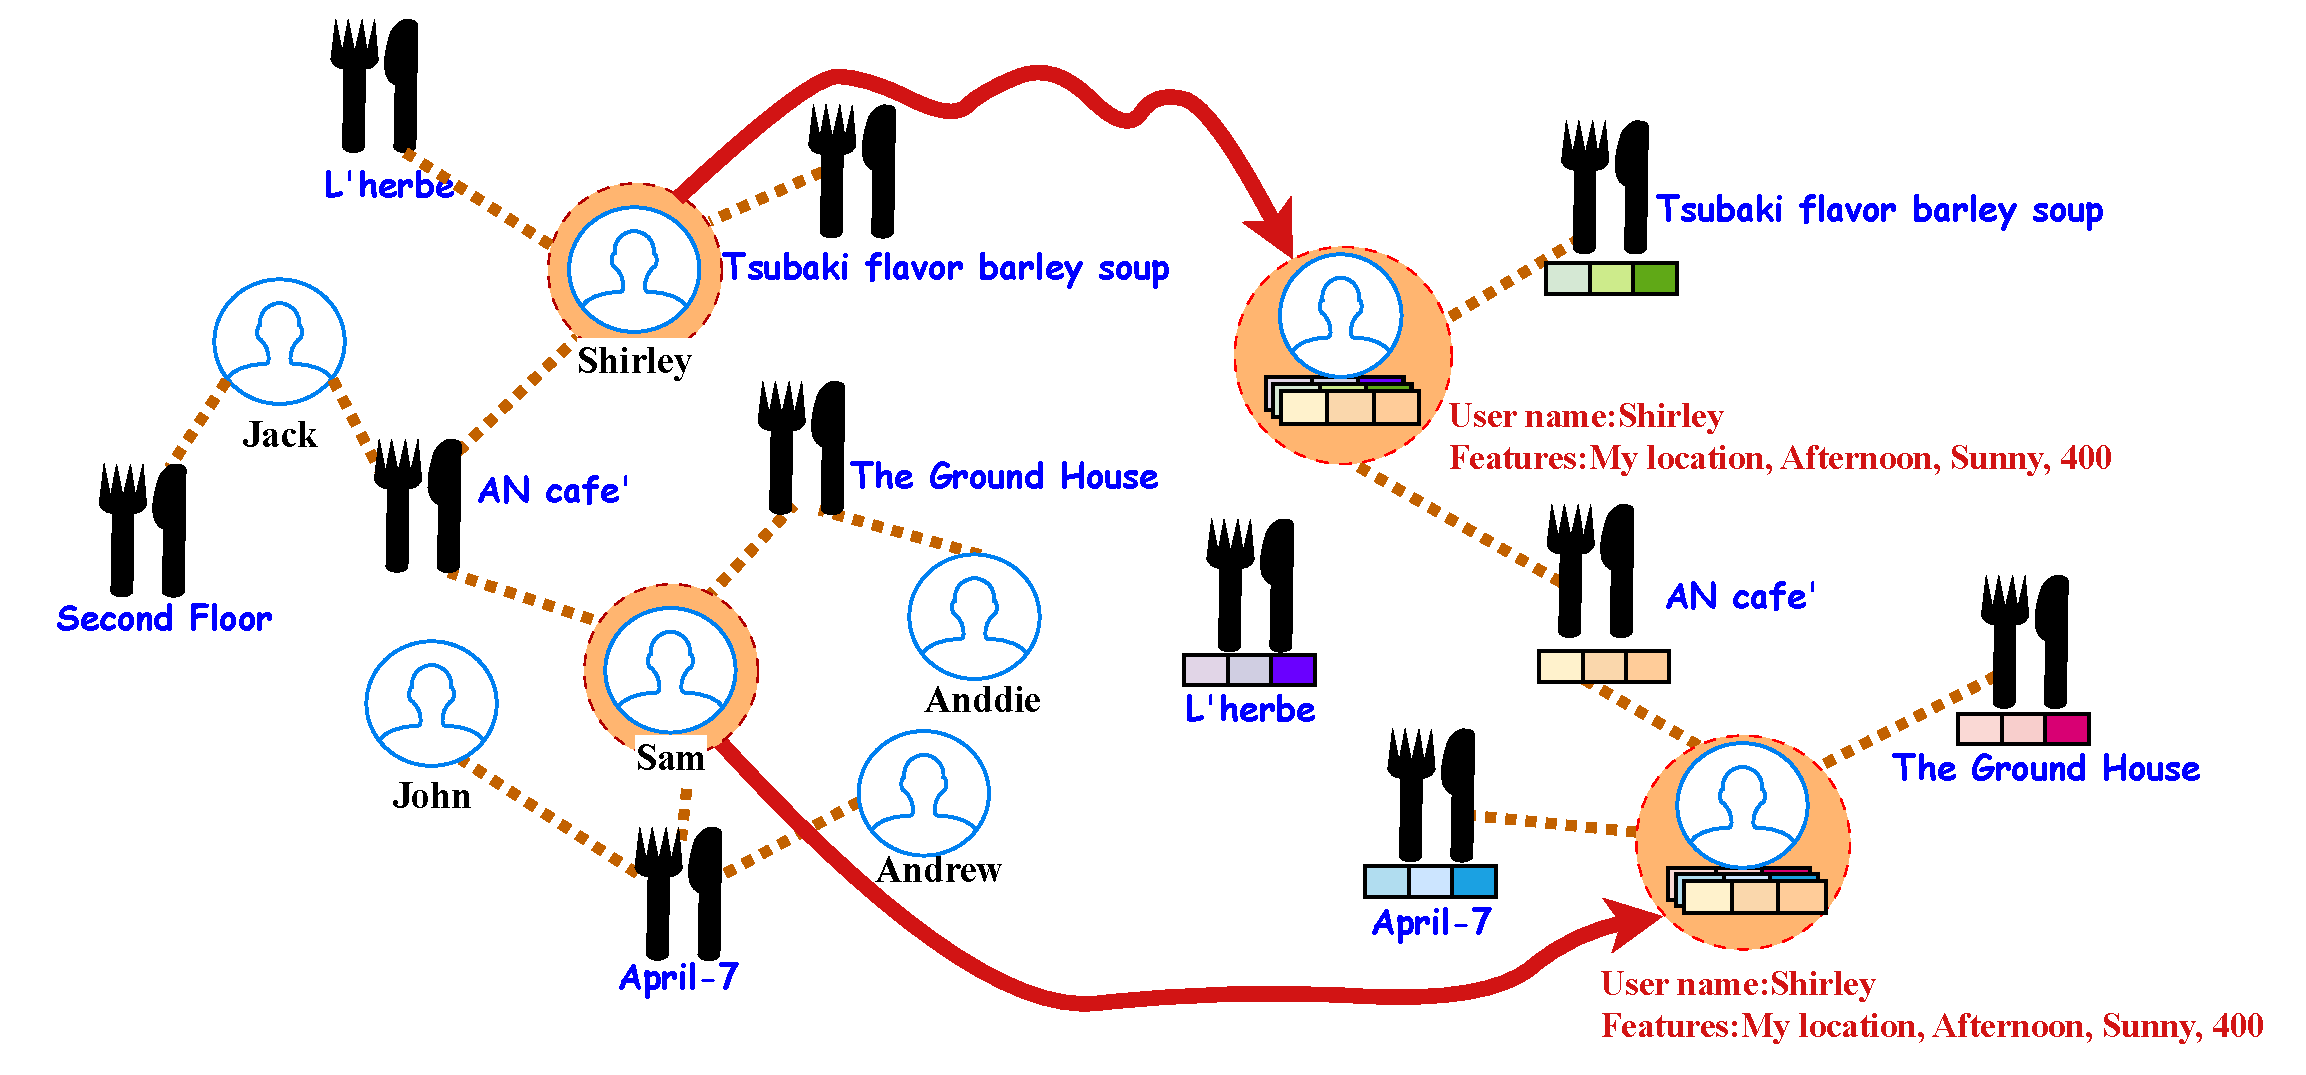
\includegraphics[width=0.48\textwidth]{img/bipartite_graph.pdf}
    \caption{二分圖於推薦系統~\cite{bipratite_fig}}
    \label{fig-bipartite}
\end{figure}
如\xfig{fig-bipartite}所示,能將所有的節點分成,左邊的使用者節點,右邊的推薦餐廳節點,因左右兩邊的節點類型不同,該圖同時為異質圖~(attributed heterogeneous graph)。
\begin{figure}[tbh]
    \centering
    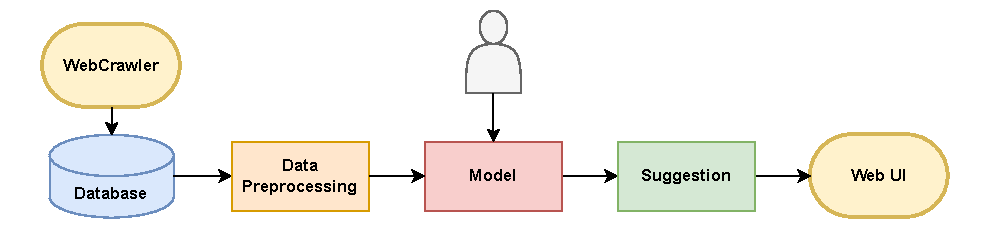
\includegraphics[width=0.5\textwidth]{img/flowg2.pdf}
    \caption{推薦系統架構圖}
    \label{fig-flowchart}
\end{figure}
本研究的架構圖如\xfig{fig-flowchart}所示,從~Foodpanda、GoogleMap~上使用爬蟲將每個店家的資訊儲存到資料庫,並使用基本的資料前處理,對於使用者節點,其節點內容如同\xtab{node-conetent},會將這些資訊同時輸入模型,並得出最後的推薦結果,再以 Web UI 的方式呈現。
\begin{table}[htbp]
    \centering
    % 調整行距
    \renewcommand{\arraystretch}{1.15}
    % 調整列間距
    \setlength{\tabcolsep}{7.5pt}
    \begin{tabular}{|c|c|}
    \hline
    \textbf{節點類型}   & \textbf{節點內容}                    \\ \hline
    使用者         & 當下位置、使用時間、天氣、預算          \\ \hline
    推薦餐廳      & 餐廳名稱、價位、評分、評論              \\ \hline
    \end{tabular}
    \caption{使用者與推薦餐廳節資訊}
    \label{node-conetent}
\end{table}
\vspace{-0.35cm}
本研究將使用 Zhang 等人所提出的圖卷機網路 \cite{NIE-GCN} 應用在店家推薦的資料集,並使用歸一化折扣累積增益~(Normalized Discounted Cumulative Gain; NDCG)~、召回率~(Recall)去衡量推薦系統之表現。




    